\documentclass[11pt,ngerman,a4paper]{article}
%Gummi|061|=)
\usepackage{amsmath}
\usepackage{a4wide}
\usepackage{url}
\usepackage{amsthm}
\usepackage{amsbsy}
\usepackage{amssymb}
\usepackage[utf8]{inputenc}
\usepackage{rotating} 
\usepackage{here}
\usepackage{graphicx}
\usepackage{paralist}
\usepackage{selinput}
\usepackage[separate-uncertainty=true]{siunitx}
\usepackage{booktabs}
\sisetup{}
\SelectInputMappings{%
adieresis={ä},
germandbls={ß},
}
\title{\textbf{Versuch V703: Geiger-Müller-Zählrohr}}
\author{Martin Bieker\\
		Julian Surmann\\
		\\
		Durchgef\"{u}hrt am 27.05.2014\\
		TU Dortmund}
\date{}
\usepackage{graphicx}
\begin{document}
\renewcommand\tablename{Tabelle}
\renewcommand\figurename{Abbildung}
\maketitle
\thispagestyle{empty}
\newpage
\clearpage
\setcounter{page}{1}


\section{Einleitung}
Das Geiger-Müller-Zählrohr ist ein einfaches Messinstrument zur Messung der Intensität von ionisierender Strahlung. In diesem Versuch werden einige Kenndaten dieer Aperatur ermittelt.
\section{Theorie}
\subsection{Aufbau und Funktion} 
 Das Geiger-M\"uller-Z\"ahlrohr besteht aus einem Draht  mit Radius $r_a$, der sich in einem Metallzylinder mit Radius $r_k$ befindet (siehe Abb \ref{}). Zwischen diesen Elementen wird eine elektische Spannung von \SI{300}{\volt} bist \SI{2000}{\volt} angelegt. Auf diese Weise entsteht zwischen Anodendraht und Kathodenzylinder ein radialsymmetrisches Feld. Der Innenraum ist mit einem  Edgasgemisch gef\"ullt. Da im Innenraum ein Unterdruck herrschen soll, ist das Z\"ahlrohr an den Enden verschlossen. An einer Seite befindet sich aber eine d\"unner Mylarfolie, damit  auch $\alpha$ und $\beta$-Teilchen in den Innenraum eindringen k\"onnen.
 
 \noindent
 Wenn Strahlung in das Z\"ahlrohrvolumen eindringt, werden die Edelgasatome ionisiert. Da die Energie der Strahlung ein Vielfaches der Ionsierungsenergie ist, k\"onnen mehrere Atome ionsiert werden, bis die Strahlung vollst\"andig absorbiert ist. Die durch die Ionisierungsakte freigesetzte Elektronen werden durch das elektrische Feld  zum Anodendraht beschleunigt.

Die nach der ersten Ionisation ablaufende Prozesse h\"anegn sehr stark von der Zylinder anliegenden Spannung ab. In Abbildung \ref{abb2} wird die Anzahl der pro einfallendem Teilchen erzeugten Elektronen-Ionen-Paare als Funktion der am Z\"ahlrohr angelegten Spannung dargestellt.

\noindent
Ist das elektrische Feld nicht sehr stark, werden rekombinieren mit den Ionen bevor sie den Anodendraht erreichen. Dies entspricht Bereich I in der Abbildung. Wird die Spannung erh\"oht erreichen mehr Elektronen den Draht bevor sie rekombinieren k\"onnen. In diesem Spannungsbereich (II in der Abbildung) wird das Z\"ahlrohr als Ionisationskammer betrieben. Bei weiterer Erh\"oung der Spannung sind  die beschleunigten Elektronen auf Grnd ihrer Energie in der Lage weitere Atome zu ionisieren. Es ensteht eine so genannte Townsend-Lawine. Es kann nun ein Ladungsimpuls gemessen werden, welcher von der Energie der Einfallenden Strahlung abh\"angt. In diesem Bereich k\"onnen mit dem Z\"ahlrohr sowohl die Intensit\"at, als auch die Energie einer Strahlungsquelle gemessen werden. Daher wird die Apparatur in diesem Bereich als Proportionalit\"atsz\"ahrohr bezeichnet. 
Steigt die Spannung weiter an, sind die Spannungsimpulse nicht mehr von der Teilchenenergie abh\"angig (Bereich IV). Bei der Ionisation durch die Elektronen enstehen auf Grund des starken elektrischen Fledes UV-Qanten. Da diese ungeladen sind, verursachen sie auf ganzer L\"ange des Z\"ahrohrs weitere Ionisationslavinen ausln\"osen. In diesem Spannungsbereich wird ein Geiger-M\"uller-Z
Bei weiterer Steigerung der Spannng wird die Apparatur durch Dauerentladungen zerst\"ort.
\subsection{Charektersitik}
Die Anzahl der Ladungsimulse bei gegebener Zeit und Quelleninensit\"at als Funktion der anliegenden Spannung wird als Charakteristik des Z\"alrohres. Diese ist beispielhaft in Abbildung \ref{abb3} dargestellt. Das in dieser Abbildung dargestellte Plateau ist der eigentliche Messsbereich des Geiger-M\"uller-Z\"ahl\"ahlrohrs.Die die L\"ange und die Steigung des Plateaus sind wichtige Kennziffern f\"ur die Qualt\"at der Apparatur.
 
\subsection{Totzeit und Nachtentladungen}

Die, bei den Ionisationsvorg\"angen entstehenden, positiven Edelgasionen haben im Vergleich zu den Elektronen eine sehr große Masse. Daher wandern diese nur langsam zur Kathode. Durch die im Zylinder vorherrschende positive Ladungsdichte schirmt das Feld indes Anodendrahts ab. Aus diesem Grund k\"onnen f\"ur eine gewisse Zeit $T$ nach einem Impuls keine weiteren Teilchen erkannnt werden. Dieser Effekt wird als Totzeit bezeichnet. Erst nachdem alle positiven Ionen neutralisiert wurden, erreichen die Ladungsimpulse ihre volle St\"arke. Dieser Zeitraum heißt Erhohlungszeit $T_E$.

\noindent
Treffen die Edelgasionen auf den Kathodenzylinder lösen diese dort Elektronen aus der Metalloberfläche. Diese Elektronen können weitere Ionisations- und Endladungslawinen auslösen. Diese Nachtentladungen verfälschen das Messergebnis, da dann bei einem Ladungsimpuls nicht unterschieden werden kann, ob dieser von einem Teilchen oder von einem Elektron aus dem Kathodenmaterial ausgelöst wurde. Um die Entstehung solcher Nachentladungen zu verhindern, wird dem Gas im Zählrohr eine geringe Menge eines Alkohols hinzugefügt. Diese relativ großen Moleküle nehmen die Engergie der Ionen auf und wandeln diese in thermische Schwingungen um. Auf diese Weise können keine Elektronen aus der Metalloberfläche ausgelöst werden.
\section{Durchführung}
Der Versuch ist wie in Abbildung \ref{aufbau} gezeigt aufgebaut. 
\subsection{Aufnahme der Charakteristik}
\subsection{Oszillographische Messung der Totzeit}
\subsection{Bestimmung der Totzeit mit der Zwei-Quellen-Methode}
\subsection{Messung der pro Teilchen freigesetzten Ladungsmenge}
\section{Auswertung}
Alle Fehler wurden mit python uncertainties errechnet.
\subsection{Aufnahme der Charakteristik}
Die gemessenen und errechneten Werte sind der Tabelle \ref{teil1} zu entnehmen. Gemessen wurde die Zählrate bei einer Spannung von $\SI{300}{\volt}$ bis $\SI{700}{\volt}$.


\begin{table}[H]
\centering
\begin{tabular}{SSSSS}
\toprule
{U[V]} &{ N} &{ t[s]} &{ $I\left[\frac{1}{s}\right]$} &{ $\sigma_{I,rel}$[\%] }\\
\midrule
300.0 & 0.0 & 100.0 & 0 & nan\\
320.0 & 13617.0 & 250.0 & 54.5+-0.5 & 0.86\\
340.0 & 11192.0 & 200.0 & 56.0+-0.5 & 0.95\\
360.0 & 11231.0 & 200.0 & 56.2+-0.5 & 0.94\\
380.0 & 11601.0 & 200.0 & 58.0+-0.5 & 0.93\\
400.0 & 11410.0 & 200.0 & 57.0+-0.5 & 0.94\\
420.0 & 11459.0 & 200.0 & 57.3+-0.5 & 0.93\\
440.0 & 11496.0 & 200.0 & 57.5+-0.5 & 0.93\\
460.0 & 11433.0 & 200.0 & 57.2+-0.5 & 0.94\\
480.0 & 11379.0 & 200.0 & 56.9+-0.5 & 0.94\\
500.0 & 11457.0 & 200.0 & 57.3+-0.5 & 0.93\\
520.0 & 11437.0 & 200.0 & 57.2+-0.5 & 0.94\\
540.0 & 11376.0 & 200.0 & 56.9+-0.5 & 0.94\\
560.0 & 11564.0 & 200.0 & 57.8+-0.5 & 0.93\\
580.0 & 11620.0 & 200.0 & 58.1+-0.5 & 0.93\\
600.0 & 11333.0 & 200.0 & 56.7+-0.5 & 0.94\\
620.0 & 11382.0 & 200.0 & 56.9+-0.5 & 0.94\\
640.0 & 11449.0 & 200.0 & 57.2+-0.5 & 0.93\\
660.0 & 11414.0 & 200.0 & 57.1+-0.5 & 0.94\\
680.0 & 11507.0 & 200.0 & 57.5+-0.5 & 0.93\\
700.0 & 11642.0 & 200.0 & 58.2+-0.5 & 0.93\\
\bottomrule
\end{tabular}
\label{teil1}
\caption{Messdaten und Fehlerangabe}
\end{table}
\noindent
Die gemessene Charakteristik ist in Abbildung \ref{plot1} zu sehen.
\begin{figure}[H]
\centering
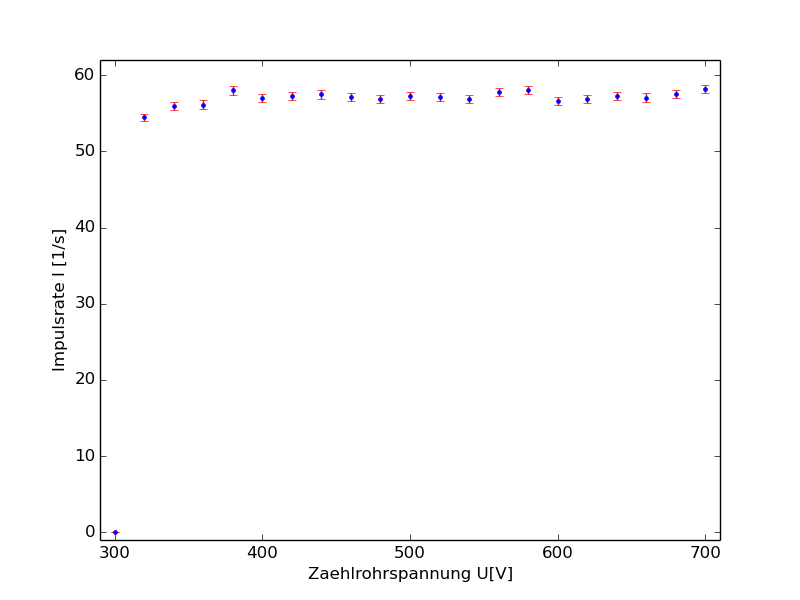
\includegraphics[scale=0.8]{plot1.png}
\label{plot1}
\end{figure}
\noindent
An diesem Plot lässt sich ablesen, dass sich das Plateaus zwischen $\SI{340}{\volt}$ und $\SI{700}{\volt}$ befindet. Im Bereich des Plateaus wird nun eine lineare Regression durchgeführt. Diese ist in Abbildung \ref{plot2} gezeigt.
\begin{figure}[H]
\centering
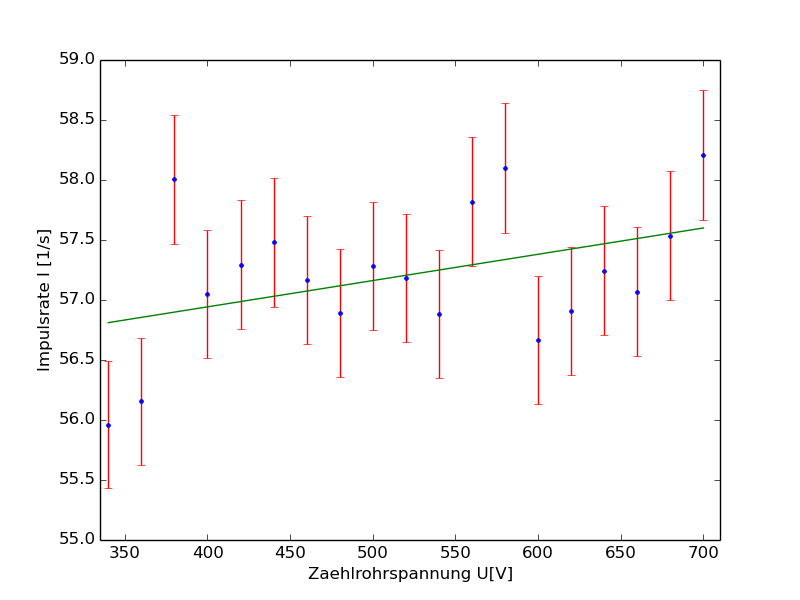
\includegraphics[scale=0.8]{plot2.png}
\label{plot2}
\end{figure}
Als Regressionsgerade ergibt sich
\[
I(U) = (0.0022\pm0.0011) \cdot U + (56.1\pm0.6).
\]
Um die Steigung des Plateaus in \% pro $\SI{100}{\volt}$ zu berechnen, sind folgende ermittelte Werte benötigt:
\begin{itemize}
\item $\Delta U = \SI{360}{\volt}$
\item $I(340) = (56.8\pm0.7) \, \frac{1}{s}$
\item $I(700) = (57.6\pm1.0) \, \frac{1}{s}$
\end{itemize}
Damit ergibt sich die Steigung zu
\[
m_I = (0.46\pm0.23) \, \frac{\%}{100\, V}.
\]
\subsection{Zeitlicher Abstand zwischen Primär- und Nachentladungsimpuls}
Es werden am Oszilloskop die Werte
\begin{itemize}
\item $\SI{195+-1}{\micro\second}$
\item $\SI{163+-1}{\micro\second}$
\end{itemize}
abgelesen.
\subsection{Oszillographische Messung der Totzeit}
Die Totzeit wurde am Oszillographen abgelesen:
\[
T_{t} = \SI{124+-30}{\micro\second}.
\]
Die Erholungszeit konnte nur grob abgeschätzt werden. Es ergab sich
\[
T_E \approx \SI{467+-30}{\micro\second}.
\]
\subsection{Bestimmung der Totzeit mit der Zwei-Quellen-Methode}
Die gemessenen Werte der Zwei-Quellen-Methode sind in Tabelle \ref{tab4} eingetragen.

\begin{table}[H]
\centering
\begin{tabular}{SSSSS}
\toprule
{Quelle} & {N} &{ t[s]} &{ $I\left[\frac{1}{s}\right]$} &{ $\sigma_{I,rel}$[\%] }\\
\midrule
1 & 17483.0 & 200.0 & 87.4+-0.7 & 0.76\\
1/2& 20229.0 & 200.0 & 101.1+-0.7 & 0.70\\
2 & 13280.0 & 1000.0 & 13.28+-0.12 & 0.87\\
\bottomrule
\end{tabular}
\label{tab4}
\caption{Zweiquellenmethode}
\end{table}

\noindent
Als Wert für die Totzeit ergibt sich
\[
T_{t} = \SI{-0.0002+-0.0004}{\second}.
\]
Dieser Wert ist negativ, weil die gemeinsame Messung der Quellen eine höhere Intensität ergab als beide Einzelmessungen addiert. Im Rahmen der Unsicherheiten ist ein positiver Wert jedoch generell möglich. Der hier gemessene Wert hat jedoch keine Aussagekraft.
\subsection{Messung der pro Teilchen freigesetzten Ladungsmenge}
Die Messwerte, die zur Bestimmung der Ladung nötig sind, sowie die Ergebnisse sind in Tabelle 3 abgebildet.

\section{Diskussion}

\section{Quellen}
\begin{enumerate}[{[}1{]}]
\item Entnommen der Praktikumsanleitung \textit{} der TU Dortmund. \\
Download am 01.06.14 unter:\\
 \url{http://129.217.224.2/HOMEPAGE/PHYSIKER/BACHELOR/AP/SKRIPT/V703.pdf}
\end{enumerate}

\section{Anhang}
\begin{itemize}
\item Tabellen
\item Auszug aus dem Messheft
\end{itemize}
\end{document}
